\subsection{Network Capacity}\label{sec:network-capacity}

The generated returns for the ForGAN baseline are reported in Tables~\ref{tab:capacity_n8} and~\ref{tab:capacity_n32}. The six configurations from Table~\ref{tab:configurations} differ in the noise dimension $N$ and the LSTM hidden sizes $R_G$ and $R_D$. All six configurations follow the training length of configuration 2, so that the effect of capacity is isolated from the training schedule. Configuration 2, examined in Sec.~\ref{sec:baseline}, is carried over for reference. Table~\ref{tab:capacity_n8} holds the noise dimension at $N = 8$, and Table~\ref{tab:capacity_n32} at $N = 32$. In Table~\ref{tab:capacity_n8}, configurations 2 and 4 differ only in $R_D$, while configurations 4 and 10 differ only in $R_G$. In Table~\ref{tab:capacity_n32}, configurations 3 and 5 differ only in $R_D$, while configurations 5 and 8 differ only in $R_G$. Comparing corresponding columns across the two tables isolates $N$.


\begin{table}[htbp]
  \centering
  \begin{tabular*}{\textwidth}{@{\extracolsep{\fill}}lrrrr@{}}
    \toprule
     & Test & Configuration 2 & Configuration 4 & Configuration 10 \\
    \midrule
    Mean               & $0.0006$  & \ms{-0.0029}{0.0019} & \ms{-0.0002}{0.0014} & \ms{0.0025}{0.0022}  \\
    Standard deviation & $0.0404$  & \ms{0.0365}{0.0034}  & \ms{0.0369}{0.0029}  & \ms{0.0368}{0.0022}  \\
    Skewness           & $0.92$    & \ms{0.19}{0.58}      & \ms{-0.09}{0.38}     & \ms{-0.14}{0.61}     \\
    Excess kurtosis    & $13.27$   & \ms{4.51}{1.52}      & \ms{7.95}{1.68}      & \ms{7.85}{3.39}      \\
    Minimum            & $-0.1749$ & \ms{-0.2234}{0.0287} & \ms{-0.3212}{0.0454} & \ms{-0.2772}{0.0539} \\
    Maximum            & $0.3229$  & \ms{0.2516}{0.0761}  & \ms{0.3254}{0.0532}  & \ms{0.2850}{0.0803}  \\
    $1\%$ quantile     & $-0.1305$ & \ms{-0.1074}{0.0162} & \ms{-0.1228}{0.0128} & \ms{-0.1160}{0.0179} \\
    $99\%$ quantile    & $0.0903$  & \ms{0.1103}{0.0163}  & \ms{0.1177}{0.0184}  & \ms{0.1131}{0.0106}  \\
    $P(|x| > 0.05)$    & $0.130$   & \ms{0.129}{0.021}    & \ms{0.120}{0.012}    & \ms{0.112}{0.015}    \\
    $P(|x| > 0.10)$    & $0.026$   & \ms{0.026}{0.008}    & \ms{0.033}{0.010}    & \ms{0.027}{0.005}    \\
    \midrule
    $C_2(1)$           & $0.289$   & \ms{0.125}{0.087}    & \ms{0.057}{0.071}    & \ms{0.206}{0.086}    \\
    $C_2(2)$           & $0.061$   & \ms{0.129}{0.055}    & \ms{0.123}{0.124}    & \ms{0.310}{0.174}    \\
    $C_2(5)$           & $0.094$   & \ms{0.164}{0.107}    & \ms{0.120}{0.092}    & \ms{0.223}{0.147}    \\
    $C_2(10)$          & $0.012$   & \ms{0.073}{0.056}    & \ms{0.079}{0.038}    & \ms{0.057}{0.045}    \\
    \bottomrule
  \end{tabular*}
  \caption{Distributional statistics and autocorrelation of generated
  daily TTF log returns on the test split, ForGAN baseline, configurations 2, 4, and 10}
  \label{tab:capacity_n8}
\end{table}

\begin{table}[htbp]
  \centering
  \begin{tabular*}{\textwidth}{@{\extracolsep{\fill}}lrrrr@{}}
    \toprule
     & Test & Configuration 3 & Configuration 5 & Configuration 8 \\
    \midrule
    Mean               & $0.0006$  & \ms{-0.0016}{0.0029} & \ms{0.0001}{0.0018}  & \ms{0.0019}{0.0034}  \\
    Standard deviation & $0.0404$  & \ms{0.0353}{0.0035}  & \ms{0.0354}{0.0031}  & \ms{0.0369}{0.0036}  \\
    Skewness           & $0.92$    & \ms{0.02}{0.68}      & \ms{0.41}{0.68}      & \ms{0.54}{0.88}      \\
    Excess kurtosis    & $13.27$   & \ms{4.70}{1.53}      & \ms{7.04}{1.83}      & \ms{10.12}{2.59}     \\
    Minimum            & $-0.1749$ & \ms{-0.2326}{0.0675} & \ms{-0.2746}{0.0978} & \ms{-0.2509}{0.0482} \\
    Maximum            & $0.3229$  & \ms{0.2478}{0.0444}  & \ms{0.3497}{0.0556}  & \ms{0.3742}{0.0535}  \\
    $1\%$ quantile     & $-0.1305$ & \ms{-0.1013}{0.0213} & \ms{-0.1007}{0.0247} & \ms{-0.1055}{0.0304} \\
    $99\%$ quantile    & $0.0903$  & \ms{0.1020}{0.0167}  & \ms{0.1130}{0.0101}  & \ms{0.1185}{0.0258}  \\
    $P(|x| > 0.05)$    & $0.130$   & \ms{0.121}{0.022}    & \ms{0.110}{0.015}    & \ms{0.104}{0.016}    \\
    $P(|x| > 0.10)$    & $0.026$   & \ms{0.021}{0.007}    & \ms{0.025}{0.009}    & \ms{0.027}{0.006}    \\
    \midrule
    $C_2(1)$           & $0.289$   & \ms{0.159}{0.097}    & \ms{0.121}{0.111}    & \ms{0.263}{0.201}    \\
    $C_2(2)$           & $0.061$   & \ms{0.121}{0.028}    & \ms{0.116}{0.099}    & \ms{0.170}{0.113}    \\
    $C_2(5)$           & $0.094$   & \ms{0.105}{0.098}    & \ms{0.132}{0.127}    & \ms{0.167}{0.112}    \\
    $C_2(10)$          & $0.012$   & \ms{0.074}{0.035}    & \ms{0.043}{0.033}    & \ms{0.144}{0.103}    \\
    \bottomrule
  \end{tabular*}
  \caption{Distributional statistics and autocorrelation of generated
  daily TTF log returns on the test split, ForGAN baseline, configurations 3, 5, and 8.}
  \label{tab:capacity_n32}
\end{table}

\textbf{Discriminator hidden size.} At both values of the noise dimension $N$, the discriminator hidden size $R_D$ has a consistent effect on the excess kurtosis of the generated returns. Increasing $R_D$ from 8 to 64 raises the excess kurtosis from \ms{4.51}{1.52} under configuration 2 to \ms{7.95}{1.68} under configuration 4 at $N = 8$, and the seed ranges of the two configurations do not overlap. At $N=32$, the excess kurtosis rises from \ms{4.70}{1.53} under configuration 3 to \ms{7.04}{1.83} under configuration 5, where the seed ranges of the two configurations overlap. Both values remain below the $13.27$ of the test split. Increasing $R_D$ also affects the largest negative returns. The minimum of the generated returns reaches \ms{-0.3212}{0.0454} under configuration 4, while the minimum of the test split is $-0.1749$. The \SI{1}{\percent} quantile, however, moves from \ms{-0.1074}{0.0162} to \ms{-0.1228}{0.0128} with overlapping seed ranges. Both of these values remain above the \SI{1}{\percent} quantile of the test split, $-0.1305$. As a result, increasing $R_D$ lowers the minimum of the generated returns, while the level below which \SI{1}{\percent} of the returns fall is not separable from the seed variation.

\textbf{Generator hidden size.} The generator hidden size $R_G$ has no separable effect on the excess kurtosis of the generated returns at either noise dimension.
At $N=8$, increasing $R_G$ from 8 to 64 changes the excess kurtosis from \ms{7.95}{1.68} under configuration 4 to \ms{7.85}{3.39} under configuration 10. The seed spread doubles, from $1.68$ to $3.39$, so the larger generator makes the training less stable without changing the mean. At $N=32$, increasing $R_G$ from 8 to 64 raises the excess kurtosis from \ms{7.04}{1.83} under configuration 5 to \ms{10.12}{2.59} under configuration 8. However, the seed ranges of the two configurations overlap.
As noted in Sec.~\ref{sec:configurations}, $R_G$ is not varied in \textcite{vuleticFinGANForecastingClassifying2024} or in the published implementation, so this comparison has no counterpart in the equity results.

\textbf{Noise dimension.} The noise dimension $N$ has no separable effect on the excess kurtosis at any of the three hidden size combinations. At $R_G = R_D = 8$, increasing $N$ from 8 to 32 changes the excess kurtosis from \ms{4.51}{1.52} under configuration 2 to \ms{4.70}{1.53} under configuration 3, with overlapping seed ranges. At $R_G = 8$ and $R_D = 64$, the excess kurtosis moves from \ms{7.95}{1.68} under configuration 4 to \ms{7.04}{1.83} under configuration 5, again with overlapping seed ranges. At $R_G = R_D = 64$, the excess kurtosis increases from \ms{7.85}{3.39} under configuration 10 to \ms{10.12}{2.59} under configuration 8, again with overlapping seed ranges.

\textbf{Configuration 8.} Configuration 8 has the highest excess kurtosis of the six configurations, \ms{10.12}{2.59}, and comes closest to the $13.27$ of the test split. The standard deviation is \ms{0.0369}{0.0036} under configuration 8, and its seed range contains the $0.0404$ of the test split. The maximum return is \ms{0.3742}{0.0535}, and its seed range contains the $0.3229$ of the test split. The probability of large returns, $P(|x|>0.10)$, is \ms{0.027}{0.006}, matching the $0.026$ for the test split. The skewness is \ms{0.54}{0.88}, against the $0.92$ of the test split, with a seed range that crosses zero. Configuration 8 does not separate from the test split on the standard deviation, the maximum or the skewness, and remains below it on the excess kurtosis.

\textbf{Volatility clustering.} None of the six configurations reproduces the decay of $C_2(\tau)$ observed in the test split. $C_2(1)$ ranges from \ms{0.057}{0.071} to \ms{0.263}{0.201} across the six configurations, against the $0.289$ of the test split. $C_2(2)$ ranges from \ms{0.116}{0.099} to \ms{0.310}{0.174}, above the $0.061$ of the test split. The values are shown in Fig.~\ref{fig:c2-capacity}. The seed spreads and the means of $C_2(\tau)$ are of the same order throughout both tables, so configurations cannot be separated from one another. As noted in Sec.~\ref{sec:baseline}, the test split is a limited reference for the shape of the decay; its own autocorrelation does not decay smoothly either. Configuration 8 is the closest to the test split at $\tau=1$, at \ms{0.263}{0.201} against $0.289$, but its $C_2(\tau)$ remains near that level at $\tau=2, 5$ and $10$.

\begin{figure}[htbp]
    \centering
    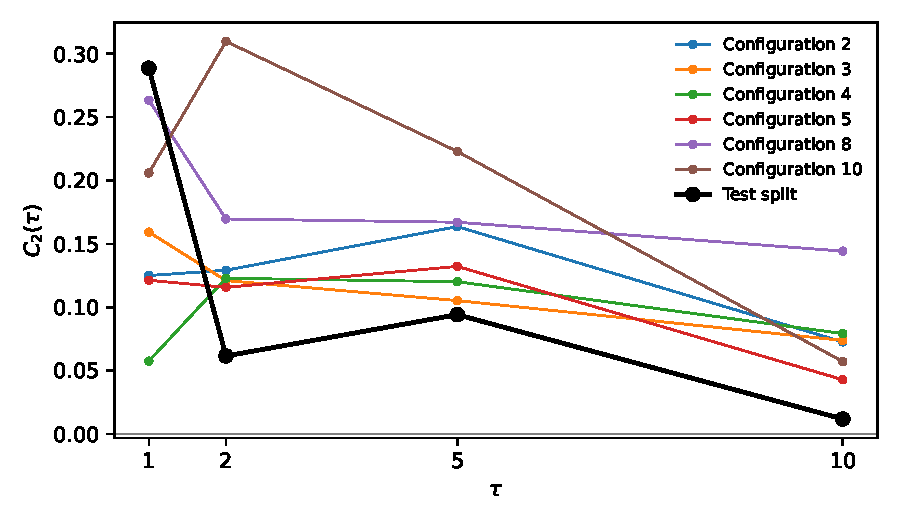
\includegraphics[width=\textwidth]{figures/c2_capacity.pdf}
    \caption{Autocorrelation of squared returns $C_2(\tau)$ for the six configurations and the test split}
    \label{fig:c2-capacity}
\end{figure}

\textbf{Training length at higher capacity.} The training length is examined further at the higher capacity settings, so the schedule of configuration 2 is no longer held fixed. Table~\ref{tab:training_length} reports the generated returns for the ForGAN baseline under configurations 7 and 9. Configurations 7 and 9 are configurations 5 and 8, respectively, with $n_{\text{epochs}} = 1500$.

The excess kurtosis of the generated returns increases from \ms{7.04}{1.83} under configuration 5 to \ms{7.97}{1.22} under configuration 7. The seed ranges overlap, so the difference in the excess kurtosis is not separable. The skewness changes from \ms{0.41}{0.68} to \ms{0.04}{0.30}, both crossing zero. The seed spreads are smaller under configuration 7 throughout the distributional statistics. As a result, a longer training schedule with a generator hidden size of $R_G = 8$ stabilizes the runs without moving them.

The excess kurtosis of the generated returns increases from \ms{10.12}{2.59} under configuration 8 to \ms{13.84}{8.77} under configuration 9. The seed ranges overlap, so the difference in the excess kurtosis is not separable. However, the mean of the excess kurtosis under configuration 9 reaches the $13.27$ of the test split. The seed spread more than triples, from $2.59$ to $8.77$, and is the largest of all configurations in this section. The skewness changes from \ms{0.54}{0.88} to \ms{1.78}{0.99}, the only skewness range among the eight configurations that does not cross zero. The skewness under configuration 9 overshoots the $0.92$ of the test split by roughly a factor of two. The maximum generated return is \ms{0.4608}{0.1127}, and its seed range excludes the $0.3229$ of the test split. $P(|x| > 0.10)$ is \ms{0.040}{0.010}, with a seed range excluding the $0.026$ of the test split. The standard deviation is \ms{0.0436}{0.0054} and its seed range contains the $0.0404$ of the test split. Configuration 9 reaches the tail weight of the test split on average and produces a reliable positive skew. However, it overshoots separably on the maximum and on $P(|x| > 0.10)$, and is the least stable of all configurations in this section.

\begin{table}[htbp]
  \centering
  \begin{tabular*}{\textwidth}{@{\extracolsep{\fill}}lrrr@{}}
    \toprule
     & Test & Configuration 7 & Configuration 9 \\
    \midrule
    Mean               & $0.0006$  & \ms{-0.0004}{0.0011} & \ms{0.0031}{0.0022}  \\
    Standard deviation & $0.0404$  & \ms{0.0368}{0.0018}  & \ms{0.0436}{0.0054}  \\
    Skewness           & $0.92$    & \ms{0.04}{0.30}      & \ms{1.78}{0.99}      \\
    Excess kurtosis    & $13.27$   & \ms{7.97}{1.22}      & \ms{13.84}{8.77}     \\
    Minimum            & $-0.1749$ & \ms{-0.3178}{0.0355} & \ms{-0.2355}{0.0246} \\
    Maximum            & $0.3229$  & \ms{0.3545}{0.0445}  & \ms{0.4608}{0.1127}  \\
    $1\%$ quantile     & $-0.1305$ & \ms{-0.1166}{0.0129} & \ms{-0.1085}{0.0082} \\
    $99\%$ quantile    & $0.0903$  & \ms{0.1163}{0.0084}  & \ms{0.1566}{0.0316}  \\
    $P(|x| > 0.05)$    & $0.130$   & \ms{0.114}{0.007}    & \ms{0.137}{0.012}    \\
    $P(|x| > 0.10)$    & $0.026$   & \ms{0.030}{0.004}    & \ms{0.040}{0.010}    \\
    \midrule
    $C_2(1)$           & $0.289$   & \ms{0.153}{0.070}    & \ms{0.160}{0.084}    \\
    $C_2(2)$           & $0.061$   & \ms{0.118}{0.088}    & \ms{0.199}{0.110}    \\
    $C_2(5)$           & $0.094$   & \ms{0.143}{0.100}    & \ms{0.115}{0.059}    \\
    $C_2(10)$          & $0.012$   & \ms{0.090}{0.058}    & \ms{0.052}{0.042}    \\
    \bottomrule
  \end{tabular*}
  \caption{Distributional statistics and autocorrelation of generated
  daily TTF log returns on the test split, ForGAN baseline, configurations 7 and 9}
  \label{tab:training_length}
\end{table}

Increasing $R_D$ from 8 to 64 is the only capacity change whose effect holds across the two tables. $R_G$ and $N$ have no separable effect on the generated returns. Of the six configurations with a fixed training schedule, configuration 8 is the closest to the test split. However, it remains below the test split on the excess kurtosis. A longer training schedule does not produce a separable change at $R_G=8$. At $R_G = 64$, a longer training schedule brings the mean of the excess kurtosis to the test split value and produces a positive skew, at the cost of stability across seeds. An increase in capacity alone does not close the gap. However, capacity combined with a longer schedule reaches the tail weight of the test split without reproducing its distribution. The condition window and the input scaling are examined in Sec.~\ref{sec:condition-window}.